\documentclass[12pt,a4paper]{article}
\usepackage[czech]{babel}
\usepackage[T1]{fontenc}
\usepackage[utf8]{inputenc}

\usepackage{graphicx} % Required for including pictures
\graphicspath{{Pictures/}} % Specifies the directory where pictures are stored

\usepackage{hyperref} % URLs
\usepackage{syntax} % Grammar typesetting
\usepackage{minted} % Program highlighting

\begin{document}

%----------------------------------------------------------------------------------------
%	TITLE PAGE
%----------------------------------------------------------------------------------------

\begin{titlepage}

\newcommand{\HRule}{\rule{\linewidth}{0.5mm}} % Defines a new command for the horizontal lines, change thickness here

\center % Center everything on the page


\includegraphics[width=0.5\textwidth]{logo-fav.png}~\\[2cm] % Include a department/university logo - this will require the graphicx package

\textsc{\Large KIV/FJP --- Semestrální práce}\\[0cm]


\HRule \\[0.8cm]
\begin{center}
 \Huge \bfseries Překladač Rustu pro LLVM\\[0.4cm] % Title of your document
\end{center}
\HRule \\[0.5cm]

\vspace{\fill}

\begin{minipage}{0.4\textwidth}
\begin{flushleft} \large
\emph{Datum:} \\
\today\\[0.2cm] % Date, change the \today to a set date if you want to be precise


\emph{Autoři:}\\
Jiří \textsc{Láska}\\
Václav \textsc{Löffelmann}\\ 
Martin \textsc{Váňa}\\[0.2cm] % Our names



\end{flushleft}
\end{minipage}
~
\begin{minipage}{0.4\textwidth}
\begin{flushright} \large


\emph{Název týmu:} \\
Falsum $\bot$\\[0.2cm] % Date, change the \today to a set date if you want to be precise

\emph{Emaily:} \\
\href{mailto:goheeca@students.zcu.cz}{goheeca@students.zcu.cz}\\
\href{mailto:loffelmv@students.zcu.cz}{loffelmv@students.zcu.cz}\\
\href{mailto:vanam@students.zcu.cz}{vanam@students.zcu.cz}\\[0.2cm] % Date, change the \today to a set date if you want to be precise


\end{flushright}
\end{minipage}\\

\end{titlepage}


%----------------------------------------------------------------------------------------
%	TOC
%----------------------------------------------------------------------------------------
\thispagestyle{empty}

\tableofcontents


\newpage


\setcounter{page}{3}

%----------------------------------------------------------------------------------------
%	TASK
%----------------------------------------------------------------------------------------

\section{Zadání}

Cílem práce bude vytvoření překladače zvoleného jazyka. Je možné inspirovat se jazykem PL/0, vybrat si podmnožinu nějakého existujícího jazyka nebo si navrhnout jazyk zcela vlastní. Dále je také potřeba zvolit si pro jakou architekturu bude jazyk překládán (doporučeny jsou instrukce PL/0, ale je možné zvolit jakoukoliv instrukční sadu pro kterou budete mít interpret).\\

\noindent
Jazyk musí mít minimálně následující konstrukce:

\begin{itemize}
	\item definice celočíselných proměnných
    \item definice celočíselných konstant
    \item přiřazení
    \item základní aritmetiku a logiku (+, -, *, /, AND, OR, negace a závorky)
    \item cyklus (libovolný)
    \item jednoduchou podmínku (\texttt{if} bez \texttt{else})
    \item definice podprogramu (procedura, funkce, metoda) a jeho volání
\end{itemize}

\noindent
Překladač který bude umět tyto základní věci bude hodnocen deseti body. Další body je možné získat na základě rozšíření, každé je za 2 body:

\begin{itemize}
    \item další typ cyklu (\texttt{for}, \texttt{do .. while}, \texttt{while .. do}, \texttt{repeat .. unitl)}
    \item \texttt{else} větev
    \item příkaz \texttt{goto} (pozor na vzdálené skoky)
    \item datový typ \texttt{boolean} a logické operace s ním
    \item datový typ \texttt{real} (s celočíselnými instrukcemi)
    \item datový typ \texttt{ratio} (s celočíselnými instrukcemi)
    \item složený datový typ (\texttt{Record})
    \item pole
    \item příkazy pro vstup a výstup (\texttt{read}, \texttt{write} - potřebuje vhodné instrukce které bude možné využít)
    \item rozvětvená podmínka (\texttt{switch}, \texttt{case})
    \item násobné přiřazení (\texttt{a = b = c = d = 3;})
    \item podmíněné přiřazení / ternární operátor (\texttt{min = (a < b) ? a : b;})
    \item paralelní přiřazení (\texttt{\{a, b, c, d\} = \{1, 2, 3, 4\};})
    \item parametry předávané odkazem
    \item parametry předávané hodnotou
    \item návratová hodnota podprogramu
    \item ...
\end{itemize}

%----------------------------------------------------------------------------------------
%	ANALYSIS
%----------------------------------------------------------------------------------------

\section{Analýza}

\begin{figure}
\centering
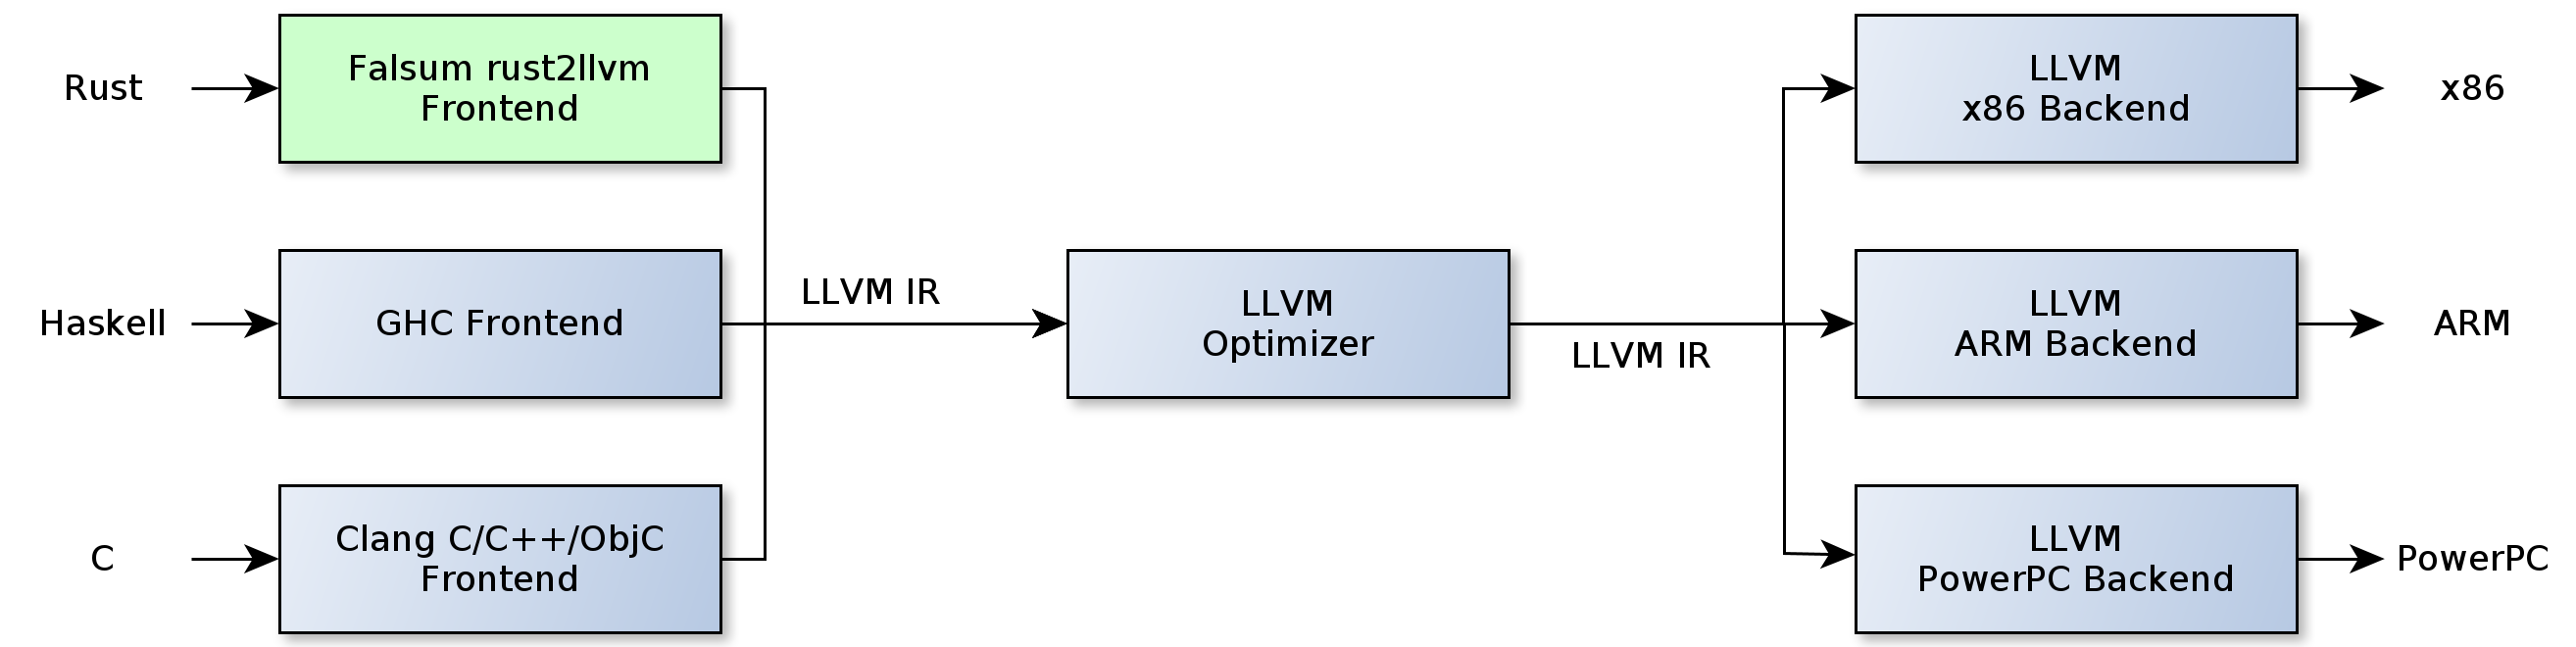
\includegraphics[width=1\textwidth]{compiler-schema.png}
\caption{Schéma překladače}
\label{img:compiler-schema}
\end{figure}

Jako zadání semestrální práce jsme si zvolili implementaci překladače podmnožiny jazyka Rust\footnote{\url{https://www.rust-lang.org/}} do mezikódu LLVM\footnote{\url{http://llvm.org/}}. 

Rust je moderní programovací jazyk, jenž si bere za cíl být srovnatelně rychlý jako C či C++ a zároveň bezpečný (ve smyslu zamezení programátorovi ve vytvoření chyb typických pro C/C++, typicky při správě paměti).

LLVM je projekt, který obsahuje mnoho nástrojů usnadňující tvorbu překladačů. LLVM IR (\textit{Intermediate Representation}) je univerzální mezijazyk, který kompilátor LLVM přeloží do spustitelné binárky pro danou platformu.

Cílem práce je tedy tvorba vlastního frontendu viz obrázek~\ref{img:compiler-schema} pro LLVM (kaskádní překladač). Z edukativních účelů jsme programovali v jazyce Haskell.\\

Pozn.: Oficiální překladač Rustu je implementován přesně tímto způsobem, ale frontend je napsaný v jazyce C.

%----------------------------------------------------------------------------------------
%	GRAMMAR
%----------------------------------------------------------------------------------------

\section{Gramatika jazyka}

\setlength{\grammarparsep}{20pt plus 1pt minus 1pt} % increase separation between rules
\setlength{\grammarindent}{12em} % increase separation between LHS/RHS 

\begin{grammar}
<Program> ::= <TopLevel> \{ <TopLevel> \}

<TopLevel> ::= <FnLet> | <ConstLet> | <IVarLet>
\alt <FVarLet> | <BinVarLet>

<FnLet> ::= `fn' <SymbolName> `(' [ <Arg> \{ `,' <Arg> \} ] `)' [ `->' <Type> ] <Block>

<Arg> ::= <SymbolName> `:' <Type>

<Block> ::= `{' \{ <Stmt> \} `}'

<Stmt> ::= <ConstLet> | <IVarLet> | <FVarLet> | <BinVarLet>
\alt <Loop> | <While> | <Return>
\alt <IIf> | <If> | <Expr> `;'

<IIf> ::= `if' <BExpr> <IIfBlock> <IElse>

<IIfBlock> ::= `{' \{ <Stmt> \} , <IExpr> | <IIf> `}'

<If> ::= `if' <BExpr> <Block> [ <Else> ]

<Expr> ::= <BExpr> | <IExpr> | <FExpr>

<Loop> ::= `loop' <Block>

<While> ::= `while' <BExpr> <Block>

<Return> ::= `return' , `;' | <IExpr> `;' | <FExpr> `;' | <BExpr> `;'

<Call> ::= <SymbolName> `(' [ <Expr> \{ `,' <Expr> \} ] `)' `;'

<Else> ::= `else' , <If> | <Block>

<IElse> ::= `else' , <IIf> | <IIfBlock>

<ConstLet> ::= `const' <SymbolName> `:' <Type> `=' <Literal> `;'

<SymbolName> ::= "isAnySymbol"

<Type> ::= `i32' | `f32' | `bool'

<Literal> ::= "intLiteral" | "floatLiteral" | <BoolLiteral>

<IVarLet> ::= <VarSymbolName> `:' `i32' `=' , <IExpr_IIf> | <IExpr> `;'

<FVarLet> ::= <VarSymbolName> `:' `f32' `=' <FExpr> `;'

<BinVarLet> ::= <VarSymbolName> [ `:' `bool' ] `=' <BExpr> `;'

<VarSymbolName> ::= `let' | `static' , <SymbolName> [ `mut' ]

<IExpr> ::= <ITerm>
\alt "OPERATOR_MAGIC(<ITerm>)" "<- `-'" "<- `*',`/',`\%'" "<- `+',`-'" "<- `&'" "<- `^'" "<- `|'"

<ITerm> ::= `(' <IExpr> `)' | <Term> | <IAssign> | <SymbolName> | <IIf> | "intLiteral"

<FExpr> ::= <FTerm>
\alt "OPERATOR_MAGIC(<FTerm>)" "<- `-'" "<-`*',`/'" "<- `+',`-'"

<FTerm> ::= `(' <FExpr> `)' | <Term> | <FAssign> | <SymbolName> | "floatLiteral"

<BExpr> ::= <BTerm>
\alt "OPERATOR_MAGIC(<BTerm>)" "<- `!'" "<- `&'" "<- `^'" "<- `|'" "<- `==',`/='" "<- `&&'" "<- `||'" 

<BTerm> ::= `(' <BExpr> `)' | <Term> | <Relation> | <BAssign> | <SymbolName> | <BoolLiteral>

<Term> ::= <Call> | <SymbolName>

<BoolLiteral> ::= `true' | `false'

<IAssign> ::= <SymbolName> `=' <IExpr>

<FAssign> ::= <SymbolName> `=' <FExpr>

<BAssign> ::= <SymbolName> `=' <BExpr>

<Relation> ::= <IExpr> <RelationOperator> <IExpr>
\alt <FExpr> <RelationOperator> <FExpr>

<RelationOperator> ::= `==' | `!=' | `<' | `>' | `<=' | `>='

\end{grammar}

%----------------------------------------------------------------------------------------
%	LANGUAGE SUBSET
%----------------------------------------------------------------------------------------

\section{Podporované jazykové konstrukce}

\subsection{Základní}

\subsubsection*{Lokální proměnné}
Proměnné musejí mít přiřazenou hodnotu při deklaraci.
\begin{minted}[autogobble]{rust}
let a: i32 = 1;
\end{minted}

\subsubsection*{Globální proměnné}

\begin{minted}[autogobble]{rust}
static M: i32 = 10;
\end{minted}

\subsubsection*{Globální konstanty}

\begin{minted}[autogobble]{rust}
const ANSWER: i32 = 42;
\end{minted}

\subsubsection*{Přiřazení}

\begin{minted}[autogobble]{rust}
a = 5;
\end{minted}

\subsubsection*{Základní aritmetika}

\begin{minted}[autogobble]{rust}
a = b + c;
a = b - c;
a = b * c;
a = b / c;
a = b & c;
a = b | c;
a = !b;
a = (a + b) * c;
\end{minted}

\subsubsection*{Nekonečný cyklus}

\begin{minted}[autogobble]{rust}
loop {...}
\end{minted}

\subsubsection*{Jednoduchá podmínka}

\begin{minted}[autogobble]{rust}
if a == 1 {...}
\end{minted}

\subsubsection*{Definice funkce}

\begin{minted}[autogobble]{rust}
fn foo() {...}
\end{minted}

\subsection{Rozšíření}

\subsubsection*{Cyklus while}

\begin{minted}[autogobble]{rust}
while a > b {...}
\end{minted}

\subsubsection*{else větev}

\begin{minted}[autogobble]{rust}
if a == 1 {...} else {...}
\end{minted}

\subsubsection*{Vícenásobná podmínka}

\begin{minted}[autogobble]{rust}
if a == 1 {...} else if a == 2 {...} else {...}
\end{minted}

\subsubsection*{Datový typ boolean a operace s ním}
Podporujeme typovou inferenci u deklarace booleanu.
\begin{minted}[autogobble]{rust}
let x: bool = true;
let y = false;

a = b & c;
a = b | c;
a = b ^ c;
a = !b;
\end{minted}

\subsubsection*{Datový typ real}

\begin{minted}[autogobble]{rust}
let x: f32 = 3.2;
\end{minted}

\subsubsection*{printf}
Příjímá variabilní počet argumentů.
\begin{minted}[autogobble]{rust}
printf("a = %d\n", a);
printf("%d %d %d\n", a, b, c);
\end{minted}

\subsubsection*{Násobné přiřazení}

\begin{minted}[autogobble]{rust}
a = b = c = d = 3
	\end{minted}

\subsubsection*{Podmíněné přiřazení}
S podmínkou umíme také pracovat jako s číselným výrazem (pokud je podmínka úplná). Může tedy sloužit například k podmíněnému přiřazení a nebo třeba jako implicitní návratová hodnota z funkce. 
Od obyčejného ifu se tento výraz liší tím, že poslední výraz v obou větvích musí být číselný a nekončící středníkem.
\begin{minted}[autogobble]{rust}
a = if a == 1 { b } else { c };
\end{minted}

\subsubsection*{Parametry předávané hodnotou}

\begin{minted}[autogobble]{rust}
fn foo(a: i32, b: bool) {...}

foo(1, true);
\end{minted}

\subsubsection*{Definice funkce s návratovou hodnotou}

\begin{minted}[autogobble]{rust}
fn bar() -> i32 {
    ...
    foo();
    ...
    retun 0;
}
\end{minted}

\noindent
Return na konci funkce je nepovinný. Pokud má funkce vracet hodnotu, může být na konci příkaz return a nebo funkce musí končit výrazem správného typu. Následující konstrukce je tedy validní.

\begin{minted}[autogobble]{rust}
fn getAnswer() -> f32 {
    42.0;
}
\end{minted}


\subsubsection*{Komentáře}

\begin{minted}[autogobble]{rust}
/*
 Víceřádkový komentář
*/

// jednořádkový
\end{minted}

\subsection{Odlišnosti od Rustu}

\subsubsection*{Deklarace proměných}

\begin{minted}[autogobble]{rust}
let a = 7;          // nepodporujeme
let a = 7i32;       // nepodporujeme
let a: i32 = 7;     // podporujeme
let b = true;       // podporujeme
let big = 1000_000; // podporujeme
\end{minted}

\subsubsection*{Mutabilita proměných}

Všechny naše proměnné jsou \textsl{mutable}.

\subsubsection*{Typové konverze}

Neimplementovali jsme typové konverze.

\subsubsection*{Výpis}

\begin{minted}[autogobble]{rust}
printf("a = %d\n", a);

// místo

println!("a = {}", a);
\end{minted}

%----------------------------------------------------------------------------------------
%	IMPLEMENTATION
%----------------------------------------------------------------------------------------

\section{Implementace}

Vlastní překlad je rozdělen do tří částí -- lexeru, parseru a generátoru kódu. Vstupem je zdrojový kód v Rustu a výstupem je mezijazyk LLVM IR, který následně přeložíme pomocí Clangu do spustitelné binárky pro danou platformu.

\subsection{Lexer}

Úkolem lexikální analýzy je převést zdrojový kód ve formě řetězce na programové symboly. K tomu jsme použili knihovnu Parsec. Lexer je poměrně obsáhlý, protože zvládá přečíst všechny lexémy v jazyce Rust i takové, které nakonec nebyly využity. Na lexikální analýzu nestačí ani konečný automat, poněvadž Rust umožňuje zadávat řetězcové literály, které jsou uvozené speciální sekvencí libovolné délky a uvnitř pak nejsou aktivní escape sekvence.

\subsection{Parser}

Parser zpracovává programové symboly a sestavuje abstraktní syntaktický strom, který předá generátoru kódu. Používá také knihovnu Parsec a vnitřně používá rekurzivní sestup. Abstraktní syntaktický strom ještě projde transformací před samotným generováním kódu. Je to příprava řetězcových konstant pro formátovací řetězce při volání funkce \em{printf}, nová funkce \em{main} s jinou signaturou atd.

\subsection{Generátor kódu}

Generátor kódu vezme abstraktní syntaktický strom a vygeneruje podle něj LLVM IR pomocí knihoven \texttt{general-llvm} a \texttt{general-llvm-pure}.

%----------------------------------------------------------------------------------------
%	USER MANUAL
%----------------------------------------------------------------------------------------

\section{Uživatelská příručka}

\subsection{Prerekvizity}

Pro přeložení a použití našeho překladače je třeba mít nainstalovano:

\begin{itemize}
	\item Haskell - \texttt{sudo apt-get install haskell-platform}
    \item The Haskell Tool Stack - \texttt{sudo apt-get install stack}
    \item Clang - \texttt{sudo apt-get install clang}
    \item LLVM - \texttt{sudo apt-get install llvm-3.8 libedit-dev}
\end{itemize}

Následně nástroj stack inicializujeme příkazem - \texttt{stack setup}

\subsection{Překlad a použití}

Aplikaci přeložíte příkazem:

\begin{center}
	\texttt{stack build}
\end{center}

\noindent
Zdrojový soubor pak přeložíte pomocí přiloženého skriptu:

\begin{center}
	\texttt{./falsum <filename>}
\end{center}

%----------------------------------------------------------------------------------------
%	EXAMPLES
%----------------------------------------------------------------------------------------

\section{Demonstrace překladače}

V této sekci se nachází několik demonstrací našeho překladače. Vždy je uveden zdrojový text v Rustu a výsledný LLVM mezikód. Více demonstrací můžete nalézt v přiloženém adresáři \texttt{/examples/}.

\subsection{Hello world}

\subsubsection{Zdrojový text}

\begin{minted}[autogobble]{rust}
fn main() {
    printf("Hello world!\n");
}
\end{minted}

\subsubsection{Mezikód}

\begin{minted}[autogobble]{llvm}
; ModuleID = '00_hello_world.rs'

@.format.0 = private global [14 x i8] c"Hello world!\0A\00", align 1

; Function Attrs: nounwind uwtable
define void @.main() #0 {
_1:
  br label %_2

_2:                                               ; preds = %_1
  %0 = call i32 (i8*, ...) @printf(
    i8* getelementptr inbounds ([14 x i8], 
    [14 x i8]* @.format.0, i32 0, i32 0))
  br label %_3

_3:                                               ; preds = %_2
  ret void
}

declare i32 @printf(i8*, ...)

; Function Attrs: nounwind uwtable
define i32 @main() #0 {
_1:
  br label %_2

_2:                                               ; preds = %_1
  call void @.main()
  br label %_3

_3:                                               ; preds = %_2
  br label %_4

_4:                                               ; preds = %_3
  ret i32 0
}

attributes #0 = { nounwind uwtable }
\end{minted}

\subsection{Základní jazykové konstrukce}

\subsubsection{Zdrojový text}

\begin{minted}[autogobble]{rust}
// global variable
static START: i32 = 10;

// constant
const DECREMENT: i32 = 1;

fn main() {
    // variables are mutable, mut keyword is optional
    let mut c: i32 = START;
    let d: i32 = 2;                // unused variable

    loop {
        printf("%d\n", c);

        c = c - DECREMENT;

        if c == 0 {
            return;
        }
    }
    // unreachable
}
\end{minted}


\subsubsection{Mezikód}

\begin{minted}[autogobble]{llvm}
; ModuleID = '{handle: 01_basic.rs}'

@START = internal global i32 10, align 4
@DECREMENT = internal global i32 1, align 4
@.format.0 = private global [4 x i8] c"%d\0A\00", align 1

; Function Attrs: nounwind uwtable
define void @.main() #0 {
_1:
  br label %_2

_2:                                               ; preds = %_1
  %c = alloca i32, align 4
  br label %_3

_3:                                               ; preds = %_2
  %0 = load i32, i32* @START, align 4
  br label %_4

_4:                                               ; preds = %_3
  store i32 %0, i32* %c, align 4
  br label %_5

_5:                                               ; preds = %_4
  %1 = load i32, i32* %c, align 4
  br label %_6

_6:                                               ; preds = %_5
  %d = alloca i32, align 4
  br label %_7

_7:                                               ; preds = %_6
  br label %_8

_8:                                               ; preds = %_7
  store i32 2, i32* %d, align 4
  br label %_9

_9:                                               ; preds = %_8
  %2 = load i32, i32* %d, align 4
  br label %_10

_10:                                              ; preds = %_9
  br label %_10_loop_1

_10_loop_1:                                       ; preds = %_10_loop_12, %_10
  %3 = load i32, i32* %c, align 4
  br label %_10_loop_2

_10_loop_2:                                       ; preds = %_10_loop_1
  %4 = call i32 (i8*, ...) @printf(
    i8* getelementptr inbounds ([4 x i8], [4 x i8]* @.format.0,
    i32 0, i32 0), i32 %3)
  br label %_10_loop_3

_10_loop_3:                                       ; preds = %_10_loop_2
  %5 = load i32, i32* %c, align 4
  br label %_10_loop_4

_10_loop_4:                                       ; preds = %_10_loop_3
  %6 = load i32, i32* @DECREMENT, align 4
  br label %_10_loop_5

_10_loop_5:                                       ; preds = %_10_loop_4
  %7 = sub i32 %5, %6
  br label %_10_loop_6

_10_loop_6:                                       ; preds = %_10_loop_5
  store i32 %7, i32* %c, align 4
  br label %_10_loop_7

_10_loop_7:                                       ; preds = %_10_loop_6
  %8 = load i32, i32* %c, align 4
  br label %_10_loop_8

_10_loop_8:                                       ; preds = %_10_loop_7
  %9 = load i32, i32* %c, align 4
  br label %_10_loop_9

_10_loop_9:                                       ; preds = %_10_loop_8
  br label %_10_loop_10

_10_loop_10:                                      ; preds = %_10_loop_9
  %10 = icmp eq i32 %9, 0
  br label %_10_loop_11

_10_loop_11:                                      ; preds = %_10_loop_10
  br i1 %10, label %_10_loop_11_then_1, label %_10_loop_12

_10_loop_11_then_1:                               ; preds = %_10_loop_11
  ret void

_10_loop_11_then_2:                               ; No predecessors!
  br label %_10_loop_12

_10_loop_12:                                      ; preds = %_10_loop_11_then_2, %_10_loop_11
  br label %_10_loop_1

_11:                                              ; No predecessors!
  ret void
}

declare i32 @printf(i8*, ...)

; Function Attrs: nounwind uwtable
define i32 @main() #0 {
_1:
  br label %_2

_2:                                               ; preds = %_1
  call void @.main()
  br label %_3

_3:                                               ; preds = %_2
  br label %_4

_4:                                               ; preds = %_3
  ret i32 0
}

attributes #0 = { nounwind uwtable }
\end{minted}

\subsection{Faktorizace složeného čísla}
\label{sec:pollard}

\subsubsection{Zdrojový text}

\begin{minted}[autogobble]{rust}
static RANDOM_SEED: i32 = 3;  // random seed = 3, other values possible

const N: i32 = 44448853;       // we assume that n is not a large prime

fn abs_val(a: i32) -> i32 {
    // if as a expression and expression as a implicit return statement
    if a > 0 {
         a
    } else {
        -a
    }
}

// returns (a * b) % c, and minimize overflow
fn mulmod(a: i32, b: i32, c: i32) -> i32 {
    let mut tmp_b: i32 = b;
    let mut x: i32 = 0;
    let mut y: i32 = a % c;

    while tmp_b > 0 {
        if tmp_b % 2 == 1 {
            x = (x + y) % c;
        }
        y = (y * 2) % c;
        tmp_b = tmp_b / 2;
    }

    return x % c;
}

fn gcd(a: i32, b: i32) -> i32 {
    // support for direct recursion
    return if b == 0 { a } else { gcd(b, a % b) };
}

fn pollard_rho(n: i32) -> i32 {
    let mut i: i32 = 0;
    let mut k: i32 = 2;

    let mut x:i32 = RANDOM_SEED;
    let mut y:i32 = RANDOM_SEED;

    let mut d: i32 = -1;

    loop {
        i = i + 1;
        x = (mulmod(x, x, n) + n - 1) % n;       // generating function

        d = gcd(abs_val(y - x), n);                  // the key insight

        // we don't support fully short-circuit operators || and &&
        // it just behave like | & respectively
        if (d != 1) & (d != n) {
            return d;
        }

        // found one non-trivial factor
        if i == k {
            y = x;
            k = k * 2;
        }
    }
    // unreachable
    return -1;                                  // set mandatory return
}

fn main() {
    // break n into two non trivial factors
    let mut ans: i32 = pollard_rho(N);
    if ans > N / ans { ans = N / ans; }  // make ans the smaller factor

    printf("%d %d\n", ans, N / ans);            // should be: 6661 6673
}

\end{minted}

\subsubsection{Mezikód}

\begin{minted}[autogobble]{llvm}
; ModuleID = '{handle: 08_complex.rs}'

@RANDOM_SEED = internal global i32 3, align 4
@N = internal global i32 44448853, align 4
@.format.0 = private global [7 x i8] c"%d %d\0A\00", align 1

; Function Attrs: nounwind uwtable
define i32 @abs_val(i32 %a) #0 {
_1:
  %0 = alloca i32, align 4
  store i32 %a, i32* %0, align 4
  br label %_2

_2:                                               ; preds = %_1
  %1 = load i32, i32* %0, align 4
  br label %_3

_3:                                               ; preds = %_2
  br label %_4

_4:                                               ; preds = %_3
  %2 = icmp sgt i32 %1, 0
  br label %_5

_5:                                               ; preds = %_4
  %.var_5 = alloca i32, align 4
  br label %_6

_6:                                               ; preds = %_5
  br i1 %2, label %_6_then_1, label %_6_else_1

_6_then_1:                                        ; preds = %_6
  %3 = load i32, i32* %0, align 4
  br label %_6_then_2

_6_then_2:                                        ; preds = %_6_then_1
  store i32 %3, i32* %.var_5, align 4
  br label %_6_then_3

_6_then_3:                                        ; preds = %_6_then_2
  br label %_7

_6_else_1:                                        ; preds = %_6
  %4 = load i32, i32* %0, align 4
  br label %_6_else_2

_6_else_2:                                        ; preds = %_6_else_1
  %5 = sub i32 0, %4
  br label %_6_else_3

_6_else_3:                                        ; preds = %_6_else_2
  store i32 %5, i32* %.var_5, align 4
  br label %_6_else_4

_6_else_4:                                        ; preds = %_6_else_3
  br label %_7

_7:                                               ; preds = %_6_else_4, %_6_then_3
  %6 = load i32, i32* %.var_5, align 4
  br label %_8

_8:                                               ; preds = %_7
  ret i32 %6
}

; Function Attrs: nounwind uwtable
define i32 @mulmod(i32 %a, i32 %b, i32 %c) #0 {
_1:
  %0 = alloca i32, align 4
  store i32 %a, i32* %0, align 4
  %1 = alloca i32, align 4
  store i32 %b, i32* %1, align 4
  %2 = alloca i32, align 4
  store i32 %c, i32* %2, align 4
  br label %_2

_2:                                               ; preds = %_1
  %tmp_b = alloca i32, align 4
  br label %_3

_3:                                               ; preds = %_2
  %3 = load i32, i32* %1, align 4
  br label %_4

_4:                                               ; preds = %_3
  store i32 %3, i32* %tmp_b, align 4
  br label %_5

_5:                                               ; preds = %_4
  %4 = load i32, i32* %tmp_b, align 4
  br label %_6

_6:                                               ; preds = %_5
  %x = alloca i32, align 4
  br label %_7

_7:                                               ; preds = %_6
  br label %_8

_8:                                               ; preds = %_7
  store i32 0, i32* %x, align 4
  br label %_9

_9:                                               ; preds = %_8
  %5 = load i32, i32* %x, align 4
  br label %_10

_10:                                              ; preds = %_9
  %y = alloca i32, align 4
  br label %_11

_11:                                              ; preds = %_10
  %6 = load i32, i32* %0, align 4
  br label %_12

_12:                                              ; preds = %_11
  %7 = load i32, i32* %2, align 4
  br label %_13

_13:                                              ; preds = %_12
  %8 = srem i32 %6, %7
  br label %_14

_14:                                              ; preds = %_13
  store i32 %8, i32* %y, align 4
  br label %_15

_15:                                              ; preds = %_14
  %9 = load i32, i32* %y, align 4
  br label %_16

_16:                                              ; preds = %_15
  br label %_16_while_1

_16_while_1:                                      ; preds = %_16_while_4_whileBody_19, %_16
  %10 = load i32, i32* %tmp_b, align 4
  br label %_16_while_2

_16_while_2:                                      ; preds = %_16_while_1
  br label %_16_while_3

_16_while_3:                                      ; preds = %_16_while_2
  %11 = icmp sgt i32 %10, 0
  br label %_16_while_4

_16_while_4:                                      ; preds = %_16_while_3
  br i1 %11, label %_16_while_4_whileBody_1, label %_17

_16_while_4_whileBody_1:                          ; preds = %_16_while_4
  %12 = load i32, i32* %tmp_b, align 4
  br label %_16_while_4_whileBody_2

_16_while_4_whileBody_2:                          ; preds = %_16_while_4_whileBody_1
  br label %_16_while_4_whileBody_3

_16_while_4_whileBody_3:                          ; preds = %_16_while_4_whileBody_2
  %13 = srem i32 %12, 2
  br label %_16_while_4_whileBody_4

_16_while_4_whileBody_4:                          ; preds = %_16_while_4_whileBody_3
  br label %_16_while_4_whileBody_5

_16_while_4_whileBody_5:                          ; preds = %_16_while_4_whileBody_4
  %14 = icmp eq i32 %13, 1
  br label %_16_while_4_whileBody_6

_16_while_4_whileBody_6:                          ; preds = %_16_while_4_whileBody_5
  br i1 %14, label %_16_while_4_whileBody_6_then_1, label %_16_while_4_whileBody_7

_16_while_4_whileBody_6_then_1:                   ; preds = %_16_while_4_whileBody_6
  %15 = load i32, i32* %x, align 4
  br label %_16_while_4_whileBody_6_then_2

_16_while_4_whileBody_6_then_2:                   ; preds = %_16_while_4_whileBody_6_then_1
  %16 = load i32, i32* %y, align 4
  br label %_16_while_4_whileBody_6_then_3

_16_while_4_whileBody_6_then_3:                   ; preds = %_16_while_4_whileBody_6_then_2
  %17 = add i32 %15, %16
  br label %_16_while_4_whileBody_6_then_4

_16_while_4_whileBody_6_then_4:                   ; preds = %_16_while_4_whileBody_6_then_3
  %18 = load i32, i32* %2, align 4
  br label %_16_while_4_whileBody_6_then_5

_16_while_4_whileBody_6_then_5:                   ; preds = %_16_while_4_whileBody_6_then_4
  %19 = srem i32 %17, %18
  br label %_16_while_4_whileBody_6_then_6

_16_while_4_whileBody_6_then_6:                   ; preds = %_16_while_4_whileBody_6_then_5
  store i32 %19, i32* %x, align 4
  br label %_16_while_4_whileBody_6_then_7

_16_while_4_whileBody_6_then_7:                   ; preds = %_16_while_4_whileBody_6_then_6
  %20 = load i32, i32* %x, align 4
  br label %_16_while_4_whileBody_6_then_8

_16_while_4_whileBody_6_then_8:                   ; preds = %_16_while_4_whileBody_6_then_7
  br label %_16_while_4_whileBody_7

_16_while_4_whileBody_7:                          ; preds = %_16_while_4_whileBody_6_then_8, %_16_while_4_whileBody_6
  %21 = load i32, i32* %y, align 4
  br label %_16_while_4_whileBody_8

_16_while_4_whileBody_8:                          ; preds = %_16_while_4_whileBody_7
  br label %_16_while_4_whileBody_9

_16_while_4_whileBody_9:                          ; preds = %_16_while_4_whileBody_8
  %22 = mul i32 %21, 2
  br label %_16_while_4_whileBody_10

_16_while_4_whileBody_10:                         ; preds = %_16_while_4_whileBody_9
  %23 = load i32, i32* %2, align 4
  br label %_16_while_4_whileBody_11

_16_while_4_whileBody_11:                         ; preds = %_16_while_4_whileBody_10
  %24 = srem i32 %22, %23
  br label %_16_while_4_whileBody_12

_16_while_4_whileBody_12:                         ; preds = %_16_while_4_whileBody_11
  store i32 %24, i32* %y, align 4
  br label %_16_while_4_whileBody_13

_16_while_4_whileBody_13:                         ; preds = %_16_while_4_whileBody_12
  %25 = load i32, i32* %y, align 4
  br label %_16_while_4_whileBody_14

_16_while_4_whileBody_14:                         ; preds = %_16_while_4_whileBody_13
  %26 = load i32, i32* %tmp_b, align 4
  br label %_16_while_4_whileBody_15

_16_while_4_whileBody_15:                         ; preds = %_16_while_4_whileBody_14
  br label %_16_while_4_whileBody_16

_16_while_4_whileBody_16:                         ; preds = %_16_while_4_whileBody_15
  %27 = sdiv exact i32 %26, 2
  br label %_16_while_4_whileBody_17

_16_while_4_whileBody_17:                         ; preds = %_16_while_4_whileBody_16
  store i32 %27, i32* %tmp_b, align 4
  br label %_16_while_4_whileBody_18

_16_while_4_whileBody_18:                         ; preds = %_16_while_4_whileBody_17
  %28 = load i32, i32* %tmp_b, align 4
  br label %_16_while_4_whileBody_19

_16_while_4_whileBody_19:                         ; preds = %_16_while_4_whileBody_18
  br label %_16_while_1

_17:                                              ; preds = %_16_while_4
  %29 = load i32, i32* %x, align 4
  br label %_18

_18:                                              ; preds = %_17
  %30 = load i32, i32* %2, align 4
  br label %_19

_19:                                              ; preds = %_18
  %31 = srem i32 %29, %30
  br label %_20

_20:                                              ; preds = %_19
  ret i32 %31
}

; Function Attrs: nounwind uwtable
define i32 @gcd(i32 %a, i32 %b) #0 {
_1:
  %0 = alloca i32, align 4
  store i32 %a, i32* %0, align 4
  %1 = alloca i32, align 4
  store i32 %b, i32* %1, align 4
  br label %_2

_2:                                               ; preds = %_1
  %2 = load i32, i32* %1, align 4
  br label %_3

_3:                                               ; preds = %_2
  br label %_4

_4:                                               ; preds = %_3
  %3 = icmp eq i32 %2, 0
  br label %_5

_5:                                               ; preds = %_4
  %.var_5 = alloca i32, align 4
  br label %_6

_6:                                               ; preds = %_5
  br i1 %3, label %_6_then_1, label %_6_else_1

_6_then_1:                                        ; preds = %_6
  %4 = load i32, i32* %0, align 4
  br label %_6_then_2

_6_then_2:                                        ; preds = %_6_then_1
  store i32 %4, i32* %.var_5, align 4
  br label %_6_then_3

_6_then_3:                                        ; preds = %_6_then_2
  br label %_7

_6_else_1:                                        ; preds = %_6
  %5 = load i32, i32* %1, align 4
  br label %_6_else_2

_6_else_2:                                        ; preds = %_6_else_1
  %6 = load i32, i32* %0, align 4
  br label %_6_else_3

_6_else_3:                                        ; preds = %_6_else_2
  %7 = load i32, i32* %1, align 4
  br label %_6_else_4

_6_else_4:                                        ; preds = %_6_else_3
  %8 = srem i32 %6, %7
  br label %_6_else_5

_6_else_5:                                        ; preds = %_6_else_4
  %9 = call i32 @gcd(i32 %5, i32 %8)
  br label %_6_else_6

_6_else_6:                                        ; preds = %_6_else_5
  store i32 %9, i32* %.var_5, align 4
  br label %_6_else_7

_6_else_7:                                        ; preds = %_6_else_6
  br label %_7

_7:                                               ; preds = %_6_else_7, %_6_then_3
  %10 = load i32, i32* %.var_5, align 4
  br label %_8

_8:                                               ; preds = %_7
  ret i32 %10
}

; Function Attrs: nounwind uwtable
define i32 @pollard_rho(i32 %n) #0 {
_1:
  %0 = alloca i32, align 4
  store i32 %n, i32* %0, align 4
  br label %_2

_2:                                               ; preds = %_1
  %i = alloca i32, align 4
  br label %_3

_3:                                               ; preds = %_2
  br label %_4

_4:                                               ; preds = %_3
  store i32 0, i32* %i, align 4
  br label %_5

_5:                                               ; preds = %_4
  %1 = load i32, i32* %i, align 4
  br label %_6

_6:                                               ; preds = %_5
  %k = alloca i32, align 4
  br label %_7

_7:                                               ; preds = %_6
  br label %_8

_8:                                               ; preds = %_7
  store i32 2, i32* %k, align 4
  br label %_9

_9:                                               ; preds = %_8
  %2 = load i32, i32* %k, align 4
  br label %_10

_10:                                              ; preds = %_9
  %x = alloca i32, align 4
  br label %_11

_11:                                              ; preds = %_10
  %3 = load i32, i32* @RANDOM_SEED, align 4
  br label %_12

_12:                                              ; preds = %_11
  store i32 %3, i32* %x, align 4
  br label %_13

_13:                                              ; preds = %_12
  %4 = load i32, i32* %x, align 4
  br label %_14

_14:                                              ; preds = %_13
  %y = alloca i32, align 4
  br label %_15

_15:                                              ; preds = %_14
  %5 = load i32, i32* @RANDOM_SEED, align 4
  br label %_16

_16:                                              ; preds = %_15
  store i32 %5, i32* %y, align 4
  br label %_17

_17:                                              ; preds = %_16
  %6 = load i32, i32* %y, align 4
  br label %_18

_18:                                              ; preds = %_17
  %d = alloca i32, align 4
  br label %_19

_19:                                              ; preds = %_18
  br label %_20

_20:                                              ; preds = %_19
  br label %_21

_21:                                              ; preds = %_20
  store i32 -1, i32* %d, align 4
  br label %_22

_22:                                              ; preds = %_21
  %7 = load i32, i32* %d, align 4
  br label %_23

_23:                                              ; preds = %_22
  br label %_23_loop_1

_23_loop_1:                                       ; preds = %_23_loop_38, %_23
  %8 = load i32, i32* %i, align 4
  br label %_23_loop_2

_23_loop_2:                                       ; preds = %_23_loop_1
  br label %_23_loop_3

_23_loop_3:                                       ; preds = %_23_loop_2
  %9 = add i32 %8, 1
  br label %_23_loop_4

_23_loop_4:                                       ; preds = %_23_loop_3
  store i32 %9, i32* %i, align 4
  br label %_23_loop_5

_23_loop_5:                                       ; preds = %_23_loop_4
  %10 = load i32, i32* %i, align 4
  br label %_23_loop_6

_23_loop_6:                                       ; preds = %_23_loop_5
  %11 = load i32, i32* %x, align 4
  br label %_23_loop_7

_23_loop_7:                                       ; preds = %_23_loop_6
  %12 = load i32, i32* %x, align 4
  br label %_23_loop_8

_23_loop_8:                                       ; preds = %_23_loop_7
  %13 = load i32, i32* %0, align 4
  br label %_23_loop_9

_23_loop_9:                                       ; preds = %_23_loop_8
  %14 = call i32 @mulmod(i32 %11, i32 %12, i32 %13)
  br label %_23_loop_10

_23_loop_10:                                      ; preds = %_23_loop_9
  %15 = load i32, i32* %0, align 4
  br label %_23_loop_11

_23_loop_11:                                      ; preds = %_23_loop_10
  %16 = add i32 %14, %15
  br label %_23_loop_12

_23_loop_12:                                      ; preds = %_23_loop_11
  br label %_23_loop_13

_23_loop_13:                                      ; preds = %_23_loop_12
  %17 = sub i32 %16, 1
  br label %_23_loop_14

_23_loop_14:                                      ; preds = %_23_loop_13
  %18 = load i32, i32* %0, align 4
  br label %_23_loop_15

_23_loop_15:                                      ; preds = %_23_loop_14
  %19 = srem i32 %17, %18
  br label %_23_loop_16

_23_loop_16:                                      ; preds = %_23_loop_15
  store i32 %19, i32* %x, align 4
  br label %_23_loop_17

_23_loop_17:                                      ; preds = %_23_loop_16
  %20 = load i32, i32* %x, align 4
  br label %_23_loop_18

_23_loop_18:                                      ; preds = %_23_loop_17
  %21 = load i32, i32* %y, align 4
  br label %_23_loop_19

_23_loop_19:                                      ; preds = %_23_loop_18
  %22 = load i32, i32* %x, align 4
  br label %_23_loop_20

_23_loop_20:                                      ; preds = %_23_loop_19
  %23 = sub i32 %21, %22
  br label %_23_loop_21

_23_loop_21:                                      ; preds = %_23_loop_20
  %24 = call i32 @abs_val(i32 %23)
  br label %_23_loop_22

_23_loop_22:                                      ; preds = %_23_loop_21
  %25 = load i32, i32* %0, align 4
  br label %_23_loop_23

_23_loop_23:                                      ; preds = %_23_loop_22
  %26 = call i32 @gcd(i32 %24, i32 %25)
  br label %_23_loop_24

_23_loop_24:                                      ; preds = %_23_loop_23
  store i32 %26, i32* %d, align 4
  br label %_23_loop_25

_23_loop_25:                                      ; preds = %_23_loop_24
  %27 = load i32, i32* %d, align 4
  br label %_23_loop_26

_23_loop_26:                                      ; preds = %_23_loop_25
  %28 = load i32, i32* %d, align 4
  br label %_23_loop_27

_23_loop_27:                                      ; preds = %_23_loop_26
  br label %_23_loop_28

_23_loop_28:                                      ; preds = %_23_loop_27
  %29 = icmp ne i32 %28, 1
  br label %_23_loop_29

_23_loop_29:                                      ; preds = %_23_loop_28
  %30 = load i32, i32* %d, align 4
  br label %_23_loop_30

_23_loop_30:                                      ; preds = %_23_loop_29
  %31 = load i32, i32* %0, align 4
  br label %_23_loop_31

_23_loop_31:                                      ; preds = %_23_loop_30
  %32 = icmp ne i32 %30, %31
  br label %_23_loop_32

_23_loop_32:                                      ; preds = %_23_loop_31
  %33 = and i1 %29, %32
  br label %_23_loop_33

_23_loop_33:                                      ; preds = %_23_loop_32
  br i1 %33, label %_23_loop_33_then_1, label %_23_loop_34

_23_loop_33_then_1:                               ; preds = %_23_loop_33
  %34 = load i32, i32* %d, align 4
  br label %_23_loop_33_then_2

_23_loop_33_then_2:                               ; preds = %_23_loop_33_then_1
  ret i32 %34

_23_loop_33_then_3:                               ; No predecessors!
  br label %_23_loop_34

_23_loop_34:                                      ; preds = %_23_loop_33_then_3, %_23_loop_33
  %35 = load i32, i32* %i, align 4
  br label %_23_loop_35

_23_loop_35:                                      ; preds = %_23_loop_34
  %36 = load i32, i32* %k, align 4
  br label %_23_loop_36

_23_loop_36:                                      ; preds = %_23_loop_35
  %37 = icmp eq i32 %35, %36
  br label %_23_loop_37

_23_loop_37:                                      ; preds = %_23_loop_36
  br i1 %37, label %_23_loop_37_then_1, label %_23_loop_38

_23_loop_37_then_1:                               ; preds = %_23_loop_37
  %38 = load i32, i32* %x, align 4
  br label %_23_loop_37_then_2

_23_loop_37_then_2:                               ; preds = %_23_loop_37_then_1
  store i32 %38, i32* %y, align 4
  br label %_23_loop_37_then_3

_23_loop_37_then_3:                               ; preds = %_23_loop_37_then_2
  %39 = load i32, i32* %y, align 4
  br label %_23_loop_37_then_4

_23_loop_37_then_4:                               ; preds = %_23_loop_37_then_3
  %40 = load i32, i32* %k, align 4
  br label %_23_loop_37_then_5

_23_loop_37_then_5:                               ; preds = %_23_loop_37_then_4
  br label %_23_loop_37_then_6

_23_loop_37_then_6:                               ; preds = %_23_loop_37_then_5
  %41 = mul i32 %40, 2
  br label %_23_loop_37_then_7

_23_loop_37_then_7:                               ; preds = %_23_loop_37_then_6
  store i32 %41, i32* %k, align 4
  br label %_23_loop_37_then_8

_23_loop_37_then_8:                               ; preds = %_23_loop_37_then_7
  %42 = load i32, i32* %k, align 4
  br label %_23_loop_37_then_9

_23_loop_37_then_9:                               ; preds = %_23_loop_37_then_8
  br label %_23_loop_38

_23_loop_38:                                      ; preds = %_23_loop_37_then_9, %_23_loop_37
  br label %_23_loop_1

_24:                                              ; No predecessors!
  br label %_25

_25:                                              ; preds = %_24
  br label %_26

_26:                                              ; preds = %_25
  ret i32 -1
}

; Function Attrs: nounwind uwtable
define void @.main() #0 {
_1:
  br label %_2

_2:                                               ; preds = %_1
  %ans = alloca i32, align 4
  br label %_3

_3:                                               ; preds = %_2
  %0 = load i32, i32* @N, align 4
  br label %_4

_4:                                               ; preds = %_3
  %1 = call i32 @pollard_rho(i32 %0)
  br label %_5

_5:                                               ; preds = %_4
  store i32 %1, i32* %ans, align 4
  br label %_6

_6:                                               ; preds = %_5
  %2 = load i32, i32* %ans, align 4
  br label %_7

_7:                                               ; preds = %_6
  %3 = load i32, i32* %ans, align 4
  br label %_8

_8:                                               ; preds = %_7
  %4 = load i32, i32* @N, align 4
  br label %_9

_9:                                               ; preds = %_8
  %5 = load i32, i32* %ans, align 4
  br label %_10

_10:                                              ; preds = %_9
  %6 = sdiv exact i32 %4, %5
  br label %_11

_11:                                              ; preds = %_10
  %7 = icmp sgt i32 %3, %6
  br label %_12

_12:                                              ; preds = %_11
  br i1 %7, label %_12_then_1, label %_13

_12_then_1:                                       ; preds = %_12
  %8 = load i32, i32* @N, align 4
  br label %_12_then_2

_12_then_2:                                       ; preds = %_12_then_1
  %9 = load i32, i32* %ans, align 4
  br label %_12_then_3

_12_then_3:                                       ; preds = %_12_then_2
  %10 = sdiv exact i32 %8, %9
  br label %_12_then_4

_12_then_4:                                       ; preds = %_12_then_3
  store i32 %10, i32* %ans, align 4
  br label %_12_then_5

_12_then_5:                                       ; preds = %_12_then_4
  %11 = load i32, i32* %ans, align 4
  br label %_12_then_6

_12_then_6:                                       ; preds = %_12_then_5
  br label %_13

_13:                                              ; preds = %_12_then_6, %_12
  %12 = load i32, i32* %ans, align 4
  br label %_14

_14:                                              ; preds = %_13
  %13 = load i32, i32* @N, align 4
  br label %_15

_15:                                              ; preds = %_14
  %14 = load i32, i32* %ans, align 4
  br label %_16

_16:                                              ; preds = %_15
  %15 = sdiv exact i32 %13, %14
  br label %_17

_17:                                              ; preds = %_16
  %16 = call i32 (i8*, ...) @printf(
    i8* getelementptr inbounds ([7 x i8], [7 x i8]* @.format.0,
    i32 0, i32 0), i32 %12, i32 %15)
  br label %_18

_18:                                              ; preds = %_17
  ret void
}

declare i32 @printf(i8*, ...)

; Function Attrs: nounwind uwtable
define i32 @main() #0 {
_1:
  br label %_2

_2:                                               ; preds = %_1
  call void @.main()
  br label %_3

_3:                                               ; preds = %_2
  br label %_4

_4:                                               ; preds = %_3
  ret i32 0
}

attributes #0 = { nounwind uwtable }
\end{minted}


%----------------------------------------------------------------------------------------
%	CONCLUSION
%----------------------------------------------------------------------------------------

\section{Závěr}

% autorův rozbor dosažených výsledků, vyzdvihnutí kladů a přínosu prezentovaného řešení,  kritika nedostatků atp.

% zhodnocení, jak bylo splněno zadání
% možnosti dalšího rozvoje prezentovaného řešení atp.

V rámci této semestrální práce byl implementován překladač, který překládá základní konstrukce naší gramatiky, jež vychází z jazyka Rust do IR LLVM. Tato základní škála bohužel neobsahuje pole, takže velká skupina algoritmů vůbec nelze vyjádřit, nicméně kromě polí nabízí tento jazyk konstrukce, na které jsou programátoři zvyklí a lze s nimi implementovat i netriviální algoritmy viz~\ref{sec:pollard}. Hlavní předností našeho řešení je striktní typová kontrola, která přidává na složitosti celého řešení.

I přes absenci podpory pro pole, semestrální práce splnila povinné body zadání a přidala velkou část z volitelných konstrukcí.

V rámci implementace jsme si v praxi vyzkoušeli funkcionální programovací jazyk Haskell a seznámili se s nástrojem LLVM, který je nápomocný při vytváření nových jazyků. Pro většinu našeho týmu byl Haskell novým jazykem, ale po úvodním seznamování jsme v něm byly schopni práci dokončit.

\end{document}
